\documentclass{book}
	\usepackage[spanish]{babel}
	%\usepackage[utf8]{inputenc}
	\usepackage[latin1]{inputenc}
	\usepackage[total={18cm,21cm},top=2cm, left=2cm]{geometry} %dise�o del documento
	\usepackage{amsmath,amssymb,amsfonts,latexsym,cancel}%paquete de texto matematico
	\usepackage[dvips]{graphicx}
	\usepackage[x11names,table]{xcolor} %paquete de colores en tablas

\begin{document}


%% Todas las palabras extranjeras con 
%% itálicas {\it texto en itálicas}

\chapter{Introducci�n}

El presente trabajo muestra el desarrollo de un sistema {\it multi-touch} %% todas las palabras extranjeras
 para crear figuras b�sicas bidimensionales.

%% Esta parte está pendiente de revisar.... no sé que es lo que decidieron al respecto.  --- va seguir existiendo las tags nadamas se simplicaron, el numero de ellas, ya es menor
La interacci�n con el sistema contar� con objetos f�sicos que representan herramientas para dibujar, adem�s se cuenta con otros objetos como herramientas b�sicas para la edici�n del dibujo. \\


El desarrollo del sistema est� enfocado en la integraci�n de tecnolog�as, 
en �ste caso particular se utilizar� la herramienta {\it Kinect}\texttrademark de {\it Microsoft}\textregistered  conectada a una computadora personal, 
adem�s el sistema contar� con reconocimiento de patrones para la selecci�n de herramientas de dibujo o de edici�n del mismo.
%%
\section{Kinect\texttrademark}

{\it Kinect}\texttrademark es un dispositivo que combina una c�mara {\it RGB}, un sensor de profundidad y un arreglo de micr�fonos\cite{Robotics}.\\

Como podemos observar en el Cuadro \ref{tab:1}, se listan los elementos principales de {\it Kinect}\texttrademark junto con su funci�n.

\begin{table}[h]
\centering
\begin{tabular}{|p{4.8cm}|p{11cm}|}
\hline
{\bf Elemento} & {\bf Funci�n}\\ \hline
Arreglo de micr�fonos& Detecta las voces y las a�sla del ruido ambiental\\ \hline
Proyector de luz infrarroja & Dispara luz infrarroja.\\ \hline
Sensor de profundidad c�mara infrarroja & Detecta la luz que lanza el proyector de luz infrarroja y genera un canal extra al {\it RGB} que trae informaci�n de la profundidad de la escena y es similar a un mapa de disparidad est�reo.\\ \hline
Motor de inclinaci�n & Ajustar hac�a donde est�n dirigidas las c�maras.\\ \hline
Salida de adaptador {\it USB} $2$.$0$ & Conectar un cable para conectar v�a {\it USB} el dispositivo.\\ \hline
C�mara {\it RGB} & Reconocer los tres colores b�sicos. Rojo, verde y azul.\\ \hline
\end{tabular}
\caption{Elementos Principales de {\it Kinect}\texttrademark \cite{ALM}.}
\label{tab:1}
\end{table}

Adem�s cuentan con:
\begin{itemize}
    \item {\it Triple Core PowerPC $970$, $3$.$2$GHz, Hyperthreaded, $2$ threads/core}.
    \item {\it $500$ MHz ATI graphics card}.
    \item {\it $512$ MB RAM}.
\end{itemize}

\section{OpenNI}

Se utiliza {\it OpenNI framework (Open Source Natural Interaction)} versi�n $1$.$3$.$4$.$6$ que es una {\it API} desarrollada por {\it OpenNI organization},  que provee una interfaz para dispositivos que ofrecen una interfaz natural para operar los componentes del {\it middleware}\cite{OpenNI}, en nuestro sistema lo utilizamos para poder comunicar la computadora personal con {\it Kinect}\texttrademark y as� utilizar de la mejor manera para lo que se dise�o el dispositivo {\it Kinect}\texttrademark, que es eliminar los dispositivos f�sicos para controlar, en este caso, la computadora personal.\\

Posee una biblioteca de c�digo abierto para poder trabajar con casi todas las capacidades de {\it Kinect}\texttrademark en {\it Windows}, {\it Linux} y {\it Mac}.

\section{OpenCV}

{\it OpenCV (Open Source Computer Vision Library)} Es una biblioteca {\it GPL}, orientada a la computaci�n visual en tiempo real, utilizada principalmente en el campo de la Interacci�n Computadora - Humano por sus siglas en ingl�s {\it HCI (Human Computer Interaction)} creada y soportada por {\it Intel} desde 1999, y tiene amplia documentaci�n.\\

Actualmente trabajamos con la versi�n $2$.$3$.$1$ de la librer�a {\it OpenCV}.\\

Una de las caracter�sticas m�s importantes de {\it OpenCV} es que las funciones est�n totalmente optimizadas para los procesadores de arquitectura {\it Intel}. Existen versiones para diferentes arquitecturas de procesadores y para diferentes sistemas operativos\cite{Intel}.

\section{Reconocimiento de Patrones}

Para intentar definir que es el Reconocimiento de Patrones (RP) definiremos algunos conceptos\cite{Theodoquidis}.\\

{\bf Reconocimiento:} Proceso de clasificaci�n de un objeto en una o m�s clases.\\

{\bf Objeto:} Es un concepto con el cual representamos los elementos sujetos a estudio. Pueden ser concretos o abstractos.\\

{\bf Patr�n:} Tras los procesos de segmentaci�n, extracci�n de caracter�sticas y descripci�n, cada objeto queda representado por una colecci�n (posiblemente ordenada y estructurada) de descriptores.\\

{\bf Clase:} Es un conjunto de objetos. Al agrupa en clases, se puede hacer de dos formas distintas:
\begin{itemize}
    \item {\it Por pertenencias duras:} Un objeto pertenece o no a una clase.
    \item {\it Por pertenencias difusas:} Los objetos pertenecen parcialmente a una clase. Existen clases con intersecciones no vac�as.
\end{itemize}

Existen varios intentos para definir al reconocimiento de patrones.
\begin{itemize}
    \item La disciplina dedicada a la clasificaci�n de objetos y el pron�stico de fen�menos.\cite{Shulcloper}
    \item Rama del conocimiento, de car�cter multidisciplinario, cuyo objeto de estudio son los procesos de identificaci�n, caracterizaci�n, clasificaci�n y reconstrucci�n sobre conjuntos de objetos o fen�menos, as� como el desarrollo de teor�as, tecnolog�as y metodolog�as relacionadas con dichos procesos.\cite{Shulcloper}
    \item Es la ciencia que se ocupa de los procesos sobre ingenier�a, computaci�n y matem�ticas relacionados con objetos f�sicos y/o abstractos, con el prop�sito de extraer informaci�n que permita establecer propiedades de o entre conjuntos de dichos objetos.\cite{Shulcloper}
\end{itemize}

Con respecto al reconocimiento de patrones, se cuenta con objetos f�sicos los cu�les  hacen la funci�n de botones permitiendo eliminar �stos de la interfaz, �stos objetos tienen asignada una imagen binaria que denominamos {\it tag}(etiqueta), as� la c�mara de {\it Kinect}\texttrademark captura la imagen del escenario, entonces el sistema procesa esa captura donde si se encuentra uno de los objetos f�sicos se decodifica la imagen y se activa la acci�n que se tenga asignada a dicha {\it tag}. Algunas de las {\it tags} tienen m�s de una acci�n que se activan con un giro en cierto �ngulo esto hace que cambie la funci�n que al principio tenia  designada.

\section{Etiquetas (Tag�s)} %% Anteriormente TAG's

Denominamos {\it tag's}(etiquetas) a un conjunto de im�genes binarias en colores blanco y negro que indica el uso de una herramienta.\\

Analizamos tres tipos de im�genes binarias candidatas, las cuales son: {\it reacTIVision fiducials}, C�digo {\it QR} y {\it ARToolKit Marker}.

\subsection{reacTIVision}

Son marcadores especiales (Figura \ref{fig:1.1}) que se desarrollaron en conjunto con el sistema {\it reacTIVision} que es un {\it software} creado especialmente para el rastreo de �stos marcadores que a grandes rasgos son im�genes binarias, espec�ficamente, en blanco y negro.

\begin{figure}[h1]
\centering
\includegraphics[scale=0.4]{ImagenesDocumentacion/reactableTag.ps}
\caption{Ejemplos de marcadores para reacTable.}
\label{fig:1.1}
\end{figure}

Para la identificaci�n de cada marcador se basa en una regi�n grafica adyacente y los rect�ngulos de delimitaci�n. El m�todo combina coincidencias de patrones binarios de gr�ficos topol�gicos (Figura \ref{fig:1.2}) para el reconocimiento y la identificaci�n con simples t�cnicas geom�tricas para calcular la ubicaci�n y orientaci�n de los marcadores\cite{Fiducials}.

\begin{figure}[h1]
\centering
\includegraphics[scale=0.7]{ImagenesDocumentacion/topologiaArbol.ps}
\caption{Algunas simples topolog�as y su correspondiente gr�fico de regi�n adyacente.}
\label{fig:1.2}
\end{figure}
\newpage
Se utilizan algoritmos gen�ticos para la identificaci�n de cada marcador, para m�s detalles consultar\cite{Fiducials}.\\

�stos marcadores est�n disponibles en PDF para su impresi�n as� como el sistema {\it reacTIVision} en la p�gina del proyecto\cite{reacTIVison} y no es necesario producir nuevos marcadores.

\subsection{C�digo QR}

El c�digo de barras de respuesta r�pida por sus siglas en ingl�s {\it QR code*}  ({\it Quick Response Barcode}, Figura \ref{fig:1.3}) es un sistema que permite almacenar informaci�n en un c�digo de barras bidimensional, esto quiere decir que tiene un patr�n de arriba hac�a abajo, de izquierda a derecha, y puede almacenar alrededor de $7,000$ d�gitos (v�ase el Cuadro \ref{tab:2}) mucho m�s que un c�digo de barras convencional, adem�s con la ayuda de una c�mara y un programa especial podemos recuperar la informaci�n de cada c�digo. �ste c�digo esta estandarizado {\it ISO/IEC 18004}.

\begin{figure}[h1]
\centering

\includegraphics[scale=0.5]{ImagenesDocumentacion/codigoQR.ps}
\caption{Ejemplo de C�digo QR.}
\label{fig:1.3}
\end{figure}

\begin{table}[h]
\centering
\begin{tabular}{|c|c|}%{|p{5cm}|p{12cm}|}%
\hline
Num�rico & M�ximo $7,089$ caracteres.\\ \hline
Alfanum�rico & M�ximo $4,296$ caracteres.\\ \hline
Binario & M�ximo $2,953$ caracteres.\\ \hline
Kanji/Kana & M�ximo $1,817$ caracteres.\\ \hline
\end{tabular}
\caption{Capacidad de datos del c�digo QR.}
\label{tab:2}
\end{table}

Existen versiones del c�digo QR desde la $1$ hasta la $40$ y cada una tiene diferentes n�meros de m�dulos (m�dulo se refiere a los puntos blancos y negros que conforman el c�digo QR)\cite{QR}.\\

\hfill{\tiny * QR code es una marca registrada por DENSO WAVE INCORPORATED}\\

Tiene la capacidad de correcci�n de errores (v�ase el Cuadro \ref{tab:3}), si una parte del c�digo est� da�ada, manchada o doblada puede ser interpretado de igual forma.

\begin{table}[h]
\centering
\begin{tabular}{|cc|}%{|p{5cm}|p{5cm}|}%
\hline
\multicolumn{2}{c}{QR Code Error Correction Capability}\\ \hline %\rowcolor{red!20}
Level L & Approx.$7\%$\\ \hline
Level M & Approx.$15\%$\\ \hline
Level Q & Approx.$25\%$\\ \hline
Level H & Approx.$30\%$\\ \hline
\end{tabular}
\caption{Capacidad de correcci�n de errores C�digo QR\cite{QR}.}
\label{tab:3}
\end{table}
\newpage
La decodificaci�n del c�digo {\it QR} puede seguir varios algoritmos a continuaci�n se describe un algoritmo general que puede utilizarse para algunos c�digo de barras  en 2D.

\begin{enumerate}
    \item Binarizaci�n de la imagen.\\
M�todo de Otsu\cite{Otsu}.
    \item Correcci�n de la inclinaci�n.
    \item Correcci�n  geom�trica  de la imagen.
    \item Obtenci�n de los cuatro v�rtices de la imagen.
    \item Obtenci�n de los nuevos valores	 de los v�rtices.
    \item Obtener el valor en cada nuevo pixel.
    \item Normalizaci�n de la imagen.
\end{enumerate}

Existen distintos sistemas que ofrecen la creaci�n de c�digos {\it QR} as� como la decodificaci�n del mismo como {\it ZXing}\cite{ZXing}.

\subsection{ARToolkit}

Son plantillas de forma cuadrada, que se componen de cuadrado negro con un cuadrado blanco cuatro veces m�s peque�o que su centro y un dibujo sencillo en el interior del cuadrado blanco, como se muestra en la  figura \ref{fig:1.4}.

\begin{figure}[h1]
\centering

\includegraphics[scale=1.5]{ImagenesDocumentacion/arToolkit.ps} 
\caption{Ejemplo de ARToolKit Marker.}
\label{fig:1.4}
\end{figure}

Para identificaci�n de la platilla est� basada en la detecci�n de las esquinas con ayuda del algoritmo de {\it fast pose estimation}\cite{ARToolkit}. Los pasos para el tratamiento de estas plantillas son los siguientes:

\begin{enumerate}
    \item La imagen capturada se transforma a una imagen binaria.
    \item Identificamos el marco de color negro.
    \item Extraemos los patrones del dibujo que se encuentra en el interior del marco negro.
    \item Almacenamos los patrones.
    \item Repetimos los primeros tres pasos.
    \item Comparamos los patrones extra�dos con los almacenados.
    \item Aplicamos  funcionalidad de la imagen.
\end{enumerate}

\section{Metodolog�a}

El desarrollo del proyecto se realiz� aplicando el modelo incremental.\cite{Pressman} %% Falta refenrencia al modelo incremental -- no falta ahi abajo esta la referencia del libro Pressman de Ing de SW 
Esta metodolog�a tiene la ventaja de ser din�mica y flexible, adem�s permite usar las salidas de las etapas precedentes, 
como entradas en las etapas sucesivas y facilita corregir cualquier error detectado o llevar a cabo mejoras en 
los distintos productos que se generan a lo largo de su aplicaci�n\cite{Pressman}.\\ 

Esta metodolog�a, se basa en la metodolog�a en cascada.El uso de esta metodolog�a dentro del desarrollo del proyecto proporcion�:
\begin{itemize}
	\item Definici�n de actividades a llevarse a cabo en el tiempo de realizaci�n del Trabajo Terminal.
	\item Unificaci�n de criterios en la organizaci�n para el desarrollo del proyecto.
	\item Puntos de control y revisi�n.
	\item Seguimiento de secuencias ascendentes o descendentes en las etapas del desarrollo.
	\item Cumplimiento de etapas o fases en paralelo, por lo que es m�s flexible que la estructurada.
\end{itemize}

\subsection{Paradigma}

El paradigma ser� Orientado a Objetos, porque la {\it API} usada de {\it OpenCV} est� en lenguaje  {\it C++}, que permite la manipulaci�n de objetos, ya que primero definen objetos, para luego enviarles mensajes solicit�ndoles que realicen sus m�todos por s� mismos.\\

El uso del paradigma proporciona:
\begin{itemize}
    \item No modela la realidad, sino la forma en que las personas comprenden y procesan la realidad.
    \item Es un proceso ascendente basado en una abstracci�n de clases en aumento.
    \item Se basa en identificaci�n de objetos, definici�n y organizaci�n de librer�as de clases, y creaci�n de macros para aplicaciones espec�ficas.
    \item Utiliza menor cantidad de c�digo.
    \item Es reutilizable.
\end{itemize}

\section{Objetivos}
\subsection{Problem�tica}
Ofrecer una alternativa al teclado y mouse con una interfaz de usuario natural donde ya no se interactu� directamente con un dispositivo electr�nico, junto con esto querer desarrollar alg�n sistema que probara que se pod�a utilizar {\it Kinect}\texttrademark junto con la computadora personal.

\subsection{General}%%
Desarrollar un sistema de interfaz de usuario natural, asistido con la herramienta de entretenimiento {\it Kinect}\texttrademark y reconocimiento de patrones. 

\subsection{Particulares} %%
\begin{itemize}
	\item Lograr una configuraci�n para usar {\it Kinect}\texttrademark con la computadora personal, para desarrollar una aplicaci�n.
	\item Eliminar uso del {\it mouse} en nuestro sistema.
	\item Eliminar uso del teclado en nuestro sistema.
	\item Reconocer una imagen binaria la cual puede ser rotada para diferentes acciones.
	\item Implementar una interfaz sin involucrar dispositivos electronicos como una pantalla tactil.
\end{itemize}

\section{Justificaci�n}

Una de las principales caracter�sticas sobre la dificultad del desarrollo de los sistemas {\it multi-touch} basado en tecnolog�a "reciente" en el caso de {\it Kinect}\texttrademark era la falta de documentaci�n fiable al momento de plantear este proyecto (Octubre - Diciembre 2011) ya que no se contaba con drivers capaces de explotar todas las caracter�sticas de {\it Kinect}\texttrademark ni un entorno de desarrollo estable por parte de {\it MS} o de la comunidad de {\it software} libre. El desarrollo de �ste sistema busca contribuir a la creaci�n de documentaci�n formal que permitir� que futuras generaciones tengan mayor cantidad de fuentes fiables y por lo tanto se interesen por la creaci�n de sistemas basados en movimientos, logrando ser un aportador m�s al crecimiento de dichos entornos.\\

Adem�s, permitir que los alumnos de la Escuela Superior de C�mputo que se encuentren cursando o tengan inter�s en el reconocimiento de patrones o semejantes, trabajen con los actuales dispositivos de captura de imagen, siendo en nuestro caso {\it Kinect}\texttrademark de {\it Microsoft}\textregistered, dejando a un lado su complejidad y crear un mayor inter�s, buscando cambiar el enfoque de dicha herramienta en donde el alumno no la vea como un proyecto de Trabajo Terminal sino como pr�cticas semestrales, lo que brindar� mayor competitividad e integraci�n de nuevas tecnolog�as.\\

Esta integraci�n de tecnolog�as ofrece una alternativa al {\it mouse} y al teclado pudiendo as� evitar enfermedades ya conocidas causadas por �stos dispositivos como lo es el s�ndrome de t�nel carpiano\cite{carpiano}. 

\subsection{Estado del arte}

Actualmente no se cuenta con un sistema de dibujo como el que se pretende realizar, a la fecha de la documentaci�n del estado del arte (Marzo 2012) existen otros trabajos que tambi�n manejan {\it Kinect\texttrademark, OpenCV y OpenNI}, elementos con los que se llevar� acabo el desarrollo de nuestro sistema, de los cuales vamos a mencionar algunos a continuaci�n.\\

Gracias a la aparici�n de {\it drivers} que permiten la interacci�n entre el dispositivo {\it Kinect}\texttrademark, que primeramente era exclusivo para la consola de videojuegos {\it Xbox} $360$ de {\it Microsoft}\textregistered, y la computadora, se comenzaron a realizar aplicaciones que permiten al usuario tener una interacci�n m�s natural, permitiendo ser ellos mismos el control de la aplicaci�n. Deb�do a que era una tecnolog�a "reciente" exist�a poca documentaci�n formal acerca de proyectos relacionados.

\subsubsection{Hand Tracking - Kinect with OpenCV 2.2 and OpenNI}

Es una aplicaci�n sencilla que en primera instancia reconoce la mano de un usuario, como  un punto permitiendo realizar trazos a mano alzada (Figura \ref{fig:1.5}), la aplicaci�n puede  cambiar el punto con que se realizar el trazo entre una mano y otra juntando las manos para volverlas a separar as� queda realizado el cambio. Esta aplicaci�n tambi�n permite la  identificaci�n del cuerpo (Figura \ref{fig:1.6}) con lo que se toman a ambas manos como puntos de  inter�s, uno de ellos se encarga de realizar el trazo y con el otro se puede seleccionar el color.

\begin{figure}[h1]
\centering
\includegraphics[0cm,0cm][18cm,6cm]{ImagenesDocumentacion/handTracking.ps} %[scale=1.5]
\caption{Hand Tracking.}
\label{fig:1.5}
\end{figure}

La relaci�n que existe entre este trabajo y el que se pens� realizar es que ambos  deben poder generar dibujos identificando un punto de interes con el cual se van a hacer los trazos adem�s de seleccionar el color y agregar otra funcionalidades. �ste sistema no cuenta con una documentaci�n y lo �nico que se puede obtener es lo que se visualiza en un video subido a la red\cite{Tracking}.

\begin{figure}[h1]
\centering
\includegraphics[0cm,0cm][16.5cm,7cm]{ImagenesDocumentacion/reconocimientoCuerpo.ps} %[scale=1.5]
\caption{Reconocimiento del cuerpo.}
\label{fig:1.6}
\end{figure}

\subsubsection{Kinect Active Projection Mapping}

Es una aplicaci�n que trabaja con {\it Kinect\texttrademark, OpenCV y OpenNI}, adem�s comparte la idea de mantener un �rea de trabajo y una proyeci�n, de tal modo el usuario interact�a directamente sobre el �rea designada (Figura \ref{fig:1.7}).\\

En este proyecto se utiliza el kinect para reconocer el cuerpo, la posici�n de las manos principalmente. El sistema crea un efecto visual en  sobre las manos y entre ellas por medio de una imagen que es proyectada sobre una pantalla detras de el usuario\cite{Mapping}.\\

Esta aplicaci�n ha sido desarrollada en el {\it Computer Fusion Laboratory} como parte del programa de ingenieria de la {\it Temple University}. La p�gina donde se dan m�s detalles del proyecto se encuentra a�n en construcci�n. Y por el momento los recursos no est�n disponibles.

\begin{figure}[h1]
\centering
\includegraphics[scale=0.8]{ImagenesDocumentacion/proyeccionManos.ps} %[0cm,0cm][16.5cm,4.5cm]
\caption{Proyecci�n de im�gen sobre un �rea de trabajo.}
\label{fig:1.7}
\end{figure}

\subsubsection{Aldebaran Nao Kinect Controller}

Es un proyecto donde se controla por medio de {\it Kinect}\texttrademark a un robot (Figura \ref{fig:1.8}), organismo aut�nomo programable y de mediana estatura desarrollado por la empresa Francesa {\it Aldebaran Robotics}. Esta aplicaci�n ha sido desarrollada en {\it Technical University Bergakademie Freiberg} en Alemania por Erik Berger y Heni Ben Amor. Existe informaci�n adicional de este proyecto en la p�gina oficial de la universidad \cite{Freiberg}, Pero se encuentra en idioma Alem�n.\\

Este proyecto no tiene mucha relaci�n en cuanto a la funcionalidad del trabajo que se desea realizar, pero se considera por el hecho de tambi�n emplear los elementos que utilizaremos en nuestro sistema. 

\begin{figure}[h1]
\centering
\includegraphics[0cm,0cm][16.5cm,7cm]{ImagenesDocumentacion/interaccionRobot.ps} %[scale=0.8]
\caption{Interacci�n con robot autom�ta programable.}
\label{fig:1.8}
\end{figure}
 %% agrega la extension .tex automaticamente
\chapter{An�lisis}

En este cap�tulo se describe el an�lisis realizado para la creaci�n del sistema.
El an�lisis se presenta seg�n los cuatro m�dulos que se reconocieron: 

\begin{enumerate}
	\item Editor B�sico de Dibujo.
	\item Reconocimiento de trazos a mano alzada.
	\item Proyecci�n sobre el �rea de trabajo.
	\item Implementaci�n de las herramientas f�sicas para el dibujo.
\end{enumerate}

Con el an�lisis correspondiente a los m�dulos tres y cuatro se fijar�n las especificaciones 
necesarias, adem�s se mencionar�n todas aquellas problem�ticas detectadas en los procesos.
Una vez que se tienen los procesos por m�dulo, se mostrar� el estudio de factibilidad que 
se realizo al correspondiente proyecto, para ver la disponibilidad de los recursos que 
necesitaron en la realizaci�n del sistema, posteriormente se expondr� la definici�n de 
requerimientos, y finalizar este cap�tulo con la especificaci�n de requerimientos.

La fase de an�lisis tiene como objetivo detectar los problemas que se puedan 
manifestar durante los procesos dentro de cada uno de los m�dulos.


%%
%% Aqu� falta una secci�n que explique como llegaron a la conclusi�n de
%% que utilizar�an cuatro m�dulos..., problablemente lo tengan en el documento de TT1.
%%


\section{M�dulo: Editor b�sico de dibujo}

Este m�dulo se encarga de realizar las tareas b�sicas dentro de una aplicaci�n de dibujo. 
Se analizaron los procesos a efectuar dentro del m�dulo y se identificaron
las siguientes tareas relacionadas al dibujo:

\begin{itemize}
 \item Trazo a mano alzada.
 \item L�nea.
 \item Circunferencia.
 \item Elipse.
 \item Pol�gono (3 a 6 lados).
\end{itemize}


\subsection{Objetivo}

Analizar los procesos necesarios para el desarrollo de un editor de dibujo y detectar 
posibles problemas por medio de la realizaci�n de pruebas que se documenten para precisar 
los requerimientos y redactar una propuesta con bases firmes y confiables.

\subsection{An�lisis y descripci�n de procesos}

A continuaci�n se describen los procesos correspondientes al m�dulo uno, 
El cuadro \ref{tab:mano_alzada} muestra el an�lisis del procedimiento de dibujo
a mano alzada. 

\begin{table}[h]
\centering
\begin{tabular}{|l|p{13cm}|} \hline
{\bf Procedimiento}:& {\bf Trazo a Mano Alzada}. \\\hline\hline
{\bf Objetivo}:&  Realizar un trazo a mano alzada, es decir a pulso. \\\hline
{\bf Descripci�n}:& Es un trazo que no requiere de reglas ni herramientas de medici�n exactas 
o auxiliares, 
s�lo con el movimiento de la mu�eca o pulso.
El trazo est�ra compuesto por varios puntos, el en�simo punto se denotar� como $P_n$ 
y el punto estar� determinado por sus dos coordenadas $P_n(x_n,y_n)$. 
Cada punto corresponde a un pixel en la pantalla. \\\hline
{\bf Datos de entrada}:& $P_n(x_n,y_n)$\\\hline
{\bf Datos de salida}:& Trazo a mano alzada. \\\hline
{\bf Problemas}:&La velocidad de desplazamiento del rat�n puede ser muy grande y,
debido a la frecuencia de muestreo del {\it hardware}, el n�mero de puntos registrados
se reduce y el trazo parecer� realizado con l�neas y no un trazo a mano alzada.\\\hline
\end{tabular}
\caption{An�lisis del proceso de dibujo a mano alzada.}
\label{tab:mano_alzada}
\end{table}


%%
%% Pendiente: Pasar estas secciones al formato del primer cuadro.
%%
\subsubsection{Trazar una L�nea recta}
Objetivo: Realizar trazos rectos a partir de dos puntos.\\\\
Descripci�n: Es la sucesi�n continua de puntos en una misma direcci�n, donde $P_1(x_1,y_1)$ es la posici�n de partida  y $P_2(x_2,y_2)$ es la posici�n final. Dados los puntos $P_1(x_1,y_1)$ y $P_2(x_2,y_2)$ se traza una l�nea entre estos por medio de la siguiente ecuaci�n.
\begin{center}
$y-y_1={(y-y_1) \over (x-x_1)}(x-x_1)$
\end{center}
Datos de entrada: $P_1(x_1,y_1)$ y $P_2(x_2,y_2)$\\\\
Datos de Salida: L�nea recta entre $P_1(x_1,y_1)$ y $P_2(x_2,y_2)$\\\\
Problemas: Se puede apreciar una peque�a deformaci�n en la l�nea, al no poder segmentar un pixel.

\subsubsection{Trazar una Circunferencia}
Objetivo: Dibujar una superficie plana limitada por una circunferencia.\\\\
Descripci�n: Es una curva cerrada y plana en la que todos sus puntos est�n a la misma distancia, de otro punto fijo, que llamamos centro. Dados los puntos $P_1(x_1,y_1)$ y $P_2(x_2,y_2)$ se traza un lugar geom�trico de los puntos de un plano que equidistan de otro punto fijo y coplanario llamado centro en una cantidad constante llamado radio.
\begin{center}
$(y-y_1)^2+(x-x_1)^2=r^2$
\end{center}
Datos de entrada: $P_1(x_1,y_1)$ y $P_2(x_2,y_2)$\\\\
Datos de salida: Circunferencia entre $P_1(x_1,y_1)$ y $P_2(x_2,y_2)$\\\\
Problemas: Se puede apreciar una deformaci�n mayo cuando la distancia entre los puntos sea menor, al ser pixeles de forma cuadrada.

\subsubsection{Trazar un Pol�gono}
Objetivo: Dibujar una figura plana compuesta por una secuencia de segmentos rectos.\\\\ 
Descripci�n: Es una figura plana compuesta por una secuencia finita de segmentos rectos consecutivos que cierran una regi�n en el espacio. Dados dos puntos $P_1(x_1,y_1)$ y $P_2(x_2,y_2)$, se genera una circunferencia  la cual se divide entre el numero de lados obteniendo as� intersecciones llamadas v�rtices, las cuales se unen atreves  de segmentos de l�nea recta.\\\\
Datos de entrada: $P_1(x_1,y_1)$ y $P_2(x_2,y_2)$\\\\
Datos de salida: Pol�gono entre $P_1(x_1,y_1)$ y $P_2(x_2,y_2)$\\\\
Problemas: Se puede apreciar una deformaci�n, cuando se le da una dimensi�n, al no poder segmentar un pixel.

\subsubsection{Trazar una elipse}
Objetivo: Es una circunferencia aplastada, una curva sim�trica cerrada. Dibujar una curva plana y cerrada, sim�trica respecto a dos ejes perpendiculares entre s�.\\\\
Descripci�n: dados los puntos  $P_1(x_1,y_1)$ y $P_2(x_2,y_2)$ se traza una curva plana cerrada que es sim�trica respecto a dos ejes, los cuales constan de focos (puntos fijos), eje focal (recta que pasa por los focos), centro (punto de intersecci�n de los focos) y de los ejes con la siguiente ecuaci�n. 	
\begin{center}
${(x-x_1)^2 \over a^2}+{(y-y_1)^2 \over b^2}=1$
\end{center}
Datos de entrada: $P_1(x_1,y_1)$ y $P_2(x_2,y_2)$\\\\
Datos de salida: Elipse  entre $P_1(x_1,y_1)$ y $P_2(x_2,y_2)$\\\\
Problemas: Se puede apreciar una deformaci�n mayor cuando la distancia entre los puntos sea menor, al ser pixeles de forma cuadrada.



\section{M�dulo: Reconocimiento de trazos a mano alzada}

Este m�dulo tiene como objetivo reconocer el trazo a mano alzada que realiza el usuario. 
El trazo del usuario ser� sensado mediante el dispotivo {\it Kinect}\texttrademark,
y deber� ser realizado en el �rea de trabajo delimitada.


%% documentar pruebas debe ir en el cap�tulo de pruebas.
%% Se documentar�n las pruebas hechas con esto corregiremos errores para cumplir con los requerimientos establecidos.


\subsection{Integraci�n del Kinect\texttrademark}
Objetivo: la computadora debe reconocer el dispositivo {\it Kinect}\texttrademark. \\\\
Descripci�n: Mediante el {\it driver OpenNI} se har� la comunicaci�n entre el dispositivo y la computadora personal, para poder realizar capturas de im�genes, utilizar y procesar la informaci�n recibida.\\\\
Datos de entrada: Datos recibidos por el sensor.\\\\
Datos de salida: Detecci�n exitosa del {\it Kinect}\texttrademark. \\\\
Problemas: No poder reconocer el dispositivo.

\subsubsection{Detecci�n de Imagen}
Objetivo: Detectar la imagen infrarroja mediante el dispositivo {\it Kinect}\texttrademark. \\\\
Descripci�n: Se capturar�n los datos de profundidad de la escena por medio de la camara infrarroja.\\\\
Datos de entrada: Datos de profundidad.\\\\
Datos de salida: Imagen de la escena con profundidad.\\\\
Problemas: Si la imagen se sale del rango para el reconocimiento no se podr� detectar.

\subsubsection{Reconocimiento del desplazamiento}
Objetivo: Detectar que un punto de inter�s realiza un desplazamiento.\\\\
Descripci�n: Mediante el {\it Kinect}\texttrademark se captura como se desplaza el punto de inter�s siguiendolo con un marcador que enfoque esa �rea.\\\\
Datos de entrada: $P_1(x_1,y_1)$\\\\
Datos de salida: $P_n(x_n,y_n)$\\\\
Problemas: si la velocidad de desplazamiento aumenta dr�sticamente se reduce la captura de los puntos.

\subsubsection{Dibujar a mano alzada con el dedo}
Objetivo: Poder plasmar el movimiento del �rea de inter�s en un trazo.\\\\
Descripci�n: Se levanta la mano y se inicia un movimiento libre dentro del rango de visi�n de {\it Kinect}\texttrademark, proces�ndolos y reflej�ndolos en el encendido de los pixeles del trazo sobre el editor.\\\\
Datos de entrada: $P_1(x_1,y_1)$\\\\
Datos de salida: $P_n(x_n,y_n)$, trazo realizado.\\\\
Problemas: Si la velocidad de desplazamiento var�a de la velocidad de procesamiento, el trazo realizado podr�a no ser igual al movimiento del dedo.

\section{M�dulo: Proyecci�n sobre el �rea de trabajo}

Este m�dulo muestra la imagen que muestra el proyector en el �rea de trabajo,
de esta manera el usuario podr� visualizar los trazos realizados.  
El an�lisis de este m�dulo requiri� probar distintas configuraciones, 
tanto del proyector como del dispositivo {\it Kinect}\texttrademark.

\subsection{Mostrar trazos realizados}
Objetivo: Poder vizualizar en el �rea de trabajo los trazos realizados.\\\\
Descripci�n: Se capturan los movimientos del dedo en una secuencia de video continuo proces�ndolos y reflej�ndolos en el encendido de los pixeles de acuerdo al trazo sobre el editor.\\\\
Datos de entrada: Secuencia de video contin�o.\\\\
Datos de salida: $P_n(x_n,y_n)$, trazo realizado.\\\\
Problemas: Si la velocidad de desplazamiento var�a de la velocidad de procesamiento, el trazo realizado podr�a no ser igual al movimiento del dedo.

\section{M�dulo 4: Implementaci�n de herramientas f�sicas}
\subsection{Introducci�n}

En la sub-secci�n siguiente, se definen los procesos que se llevan a cabo en el modulo 4, en el cual se implementan las {\it tags}, con las que el usuario puede realizar  un trazo � hacer cambios en el dibujo, dichas opciones de edici�n son: cambiar de color, mover de posici�n y escalar el dibujo. As� como detectar los problemas  que surjan en los procesos.

\subsection{Objetivo}

Analizar los procesos involucrados para el reconocimiento de las {\it tags} aplicado lo investigado sobre distintos algoritmos para reconocer la imagen binaria elegida y tener una implementaci�n completa de acuerdo a los requerimientos.

\subsection{An�lisis y descripci�n de procesos}

Este apartado describe los procesos correspondientes al desarrollo del m�dulo cuatro.

\subsubsection{Selecci�n de herramienta de trabajo}
Objetivo: Identificar la {\it tag} colocada para iniciar un trazo o la edici�n de un dibujo.\\\\
Descripci�n: Se captura imagen de la {\it tag} y se procesa, de acuerdo a que {\it tag} este colocada se internamente se selcciona la opci�n correspondiente para iniciar el trazo de un dibujo o la edici�n del mismo.\\\\
Datos de entrada: Secuencia de video continuo.\\\\
Datos de salida: No hay datos de salida visibles al usuario, internamente queda seleccionada una opci�n.\\\\
Problemas: La {\it tag} puede no estar posicionada correctamente para su identificaci�n.

\section{Estudio de Factibilidad}

Despu�s de analizar los m�dulos del sistema, el estudio de factibilidad
permiti� confirmar la disponibilidad de los recursos necesarios
para llevar a cabo este trabajo terminal. Se revisaron tres aspectos
de la factibidad, la operativa, la t�cnica y la econ�mica. 
En todos ellos se concluyo que la realizaci�n de este trabajo terminal es 
{\bf factible}. Las siguientes secciones detallan el an�lisis realizado.


%% Referencia ??
%%http://www.slideshare.net/Yuyo-R10/factibilidad-tecnica-operativa-y-economica-11765760#btnNext

\subsection{Factibilidad operativa}

%% Requerimiento de la aplicaci�n: f�cil uso. Que la aplicaci�n sea f�cil de usar.
%% C�mo se mide la facilidad de uso de una aplicaci�n?

Para determinar en que grado el sistema se utilizar� y operar� como se planea se 
realizaron .... 
%% encuestas? revisi�n de art�culos? estad�sticas??

\subsection{Factibilidad t�cnica}

Para realizar el sistema se dectaron las siguientes necesidades:
\begin{itemize}
 \item {\it Hardware}:
  \begin{itemize}
   \item Sensor {\it Kinect}\texttrademark.
   \item Proyector de video. 
   \item Equipo de c�mputo con capacidad de ejecutar los diferentes
programas y soportar la velocidad de comunicaci�n con el sensor {\it Kinect}\texttrademark y
el proyector de video.
  \end{itemize}
 \item {\it Software}:
   \begin{itemize}
    \item Sistema operativo.
    \item Entorno de programaci�n.
    \item De oficina.
   \end{itemize}
\end{itemize}

Todos estos requerimientos se satisfacen dado que, el equipo de trabajo cuenta con tres 
computadora port�tiles ({\it laptops}) y un dispositivo {\it Kinect}\texttrademark,
adem�s de que la Escuela Superior de Computo (E.S.COM.) prestar� el proyector.

Los equipos de c�mputo se utilizaron para desarrollar y hacer pruebas colectivamente con 
el dispositivo {\it Kinect}\texttrademark.

De acuerdo a la tecnolog�a necesaria para la implementaci�n del Sistema se evalu� bajo dos enfoques: {\it hardware y software}.\\\\ 

En cuanto a {\it hardware}  existente, no se requiri� realizar inversi�n inicial 
para la adquisici�n del mismo, ya que con lo que se contaba satisfac�a 
los requerimientos establecidos, tanto para el desarrollo y puesta en 
funcionamiento del sistema propuesto.

A continuaci�n se muestra  la descripci�n de las computadoras personales (Cuadros \ref{tab:2.1}, \ref{tab:2.2} y \ref{tab:2.3}) que se utilizaron para la realizaci�n del sistema, asi como las caracteristicas del kinect(Cuadro \ref{tab:2.4}):

\begin{itemize}
    \item Una {\it Apple MacBook} 
\end{itemize}

\begin{table}[h]
\centering
\begin{tabular}{|c|c|}
\hline
Procesador & Intel Core 2 Duo\\ \hline
Velocidad del Procesador & $2.26$ GHz\\ \hline
Numero de Procesadores & $1$\\ \hline
Memoria RAM & $2$ GB\\ \hline
\end{tabular}
\caption{Descripci�n t�cnica Apple MacBook.}
\label{tab:2.1}
\end{table}

\begin{itemize}
    \item Una {\it Dell Inspiron} $1545$ 
\end{itemize}

\begin{table}[h]
\centering
\begin{tabular}{|c|c|}
\hline
Procesador & Pentium Dual-Core\\ \hline
Velocidad del Procesador & $2.20$ GHz\\ \hline
Numero de Procesadores & $1$\\ \hline
Memoria RAM & $3$ GB\\ \hline
\end{tabular}
\caption{Descripci�n t�cnica Dell Inspiron m�delo 1545.}
\label{tab:2.2}
\end{table}

\begin{itemize}
    \item Una {\it HP Pavilion dv4} 
\end{itemize}

\begin{table}[h]
\centering
\begin{tabular}{|c|c|}
\hline
Procesador & AMD Athlon II Dual Core\\ \hline
Velocidad del Procesador & $2.00$ GHz\\ \hline
Numero de Procesadores & $1$\\ \hline
Memoria RAM & $3$ GB\\ \hline
\end{tabular}
\caption{Descripci�n t�cnica HP Pavillion m�delo dv4.}
\label{tab:2.3}
\end{table}
\newpage
\begin{itemize}
    \item Dispositivo {\it Kinect}\texttrademark 
\end{itemize}

\begin{table}[h]
\centering
\begin{tabular}{|c|}
\hline
Triple Core PowerPC $970$, $3.2$GHz, Hyperthreaded, $2$ threads/core.\\ \hline
$500$ MHz ATI graphics card.\\ \hline
$512$ MB RAM\\ \hline
Arreglo de micr�fonos\\ \hline
Proyector de luz infrarroja\\ \hline
Sensor de profundidad c�mara infrarroja\\ \hline
Motor de inclinaci�n\\ \hline
Salidad de adapatador USB\\ \hline
Camara RGB\\ \hline
\end{tabular}
\caption{Descripci�n t�cnica Kinect\cite{ALM}.}
\label{tab:2.4}
\end{table}

\subsection{Software actual}
En cuanto  al software, no amerita una inversi�n alguna, ya que el sistema operativo, el  {\it driver} y la {\it API} son versiones libres, las versiones que se utlizar�n se mencionan en el Cuadro \ref{tab:2.5}:

\begin{table}[h]
\centering
\begin{tabular}{|c|c|}
\hline
Sistema operativo: & Linux Ubuntu $11.04$ y versiones posteriores\\ \hline
Driver: & OpenNI versi�n $1.3.4.6$\\ \hline
API para visi�n por computadora: & OpenCv versi�n $2.3.1$\\ \hline
\end{tabular}
\caption{Software para el desarrollo del proyecto.}
\label{tab:2.5}
\end{table}

\subsubsection{Comparativa de Sistemas Operativos (S.O)}
En cu�nto al sistema operativo,se hiz�  una tabla comparativa(Cuadro \ref{tab:2.6}) de 3 sistemas diferrentes, {\it Windows 7, Ubuntu(Linux) y MacOSX}, donde se  notan las herramientas,driver, API�s y lenguajes que pueden ser usados en cada sistema, y  ver cu�l se acopla a lo que se har�, asi como al API y driver seleccionados.

\begin{table}[h]
\centering
\begin{tabular}{|p{1.7cm}|p{1.4cm}|p{2cm}|p{3cm}|p{2.5cm}|p{3cm}|}
\hline
Sistema Operativo & Driver OpenNi & Middleware o utilidades & IDE & Lenguaje & API para visi�n por computadora\\ \hline
Windows 7 & \checkmark & Nite & Visual Studio 2008 en adelante, Eclipse, CodeBlocks & C ++, Phyton & Processing\\ \hline
Ubuntu & \checkmark & Nite & QT, Eclipse, (Otros IDE's ) & C ++, Phyton & OpenCV\\ \hline
Mac OSX & \checkmark & Nite & XCode & C ++, Phyton & OpenCV\\ \hline
\end{tabular}
\caption{Comparativa entre sistemas operativos para desarrollar el proyecto.}
\label{tab:2.6}
\end{table}
\newpage
\subsubsection{Windows vs Ubuntu (Linux)}
Al tener esta comparativa  de los sistemas operativos, se empez�  a descartar opciones, para lo cual el sistema de {\it Mac} fue el primero, ya que  los equipos de computo con los que se contaba, solo se ten�a un equipo de {\it Mac}, por lo cual se  hizo otra tabla (Cuadro \ref{tab:2.7})  con las caracter�sticas de los otros dos sistemas, y ver cual ten�a m�s ponderaci�n.

\begin{table}[h]
\centering
\begin{tabular}{|c|c|c|}
\hline
Caracter�stica & Windows & Linux Ubuntu\\ \hline
Familiaridad & Si & Si\\ \hline
Seguridad & No & Si\\ \hline
Precio & No & Si\\ \hline
Drivers & Si & Si\\ \hline
\end{tabular}
\caption{Comparativa entre Windows y Ubuntu.}
\label{tab:2.7}
\end{table} 

En conclusi�n se utilizar� la distribuci�n {\it Ubuntu} del sistema operativo {\it Linux}, ya que es un software libre y no requiere de herramientas propietarias; el {\it Driver OpenNi} que nos proporciona el middleware Nite, el cual es soportado por la empresa {\it PRIMESENSE}, la cual desarrollo el dispositivo {\it Kinect}\texttrademark  y  {\it OpenCv} que es una {\it API}  para visi�n por computadora y se utilizado en proyectos con {\it Kinect}\texttrademark.

\subsection{Factibilidad Econ�mica}


%% Hace falta llenar este apartado...


\section{Requerimientos}

El an�lisis de los requerimientos permite establer aquellas 
caracter�sticas que se dise�ar�n en la siguiente etapa.
%% Referencia???
Para este trabajo terminal se identificaron los siguientes requerimientos
%% Funcionales, no funcionales???

R1: El m�dulo 1 del sistema permite dibujar a mano alzada.\\\\
R2: El m�dulo 1 del sistema permite dibujar l�neas de diferente longitud.\\\\
R3: El m�dulo 1 del sistema permite crear l�neas en diferente direcci�n (ubicaci�n).\\\\ 
R4: El m�dulo 1 del sistema permite dibujar c�rculos de diferente circunferencia.\\\\
R5: El m�dulo 1 del sistema permite dibujar una elipse de distintas dimensiones.\\\\ 
R6: El m�dulo 1 del sistema permite dibujar pol�gonos de diferentes tama�os.\\\\
R7: El m�dulo 1 del sistema permite dibujar pol�gonos de 3 a 6 lados dependiendo de la {\it tag} utilizada.\\\\
R8: El m�dulo 2 del sistema permite la integraci�n con {\it Kinect}\texttrademark.\\\\
R9: El m�dulo 2 del sistema permite la detecci�n del dedo �ndice.\\\\
R10: El m�dulo 2 del sistema permite reconocer el desplazamiento del dedo �ndice.\\\\
R11: El m�dulo 2 del sistema permite dibujar a mano alzada con el dedo �ndice.\\\\
R12: El m�dulo 2 del sistema permite proyectar en el editor b�sico de dibujo la acci�n realizada por el dedo �ndice.\\\\
R13: El m�dulo 3 del sistema permite  trabajar conjuntamente proyector y {\it Kinect}\texttrademark.\\\\
R14: El m�dulo 3 del sistema permite proyectar sobre el �rea de trabajo.\\\\
R15: El m�dulo 3 del  sistema permite trabajar  sin interferencia de la sombra que produzca la mano.\\\\
R16: El m�dulo 4 del sistema permite reconocer la herramienta ({\it tag}).\\\\
R17: El m�dulo 4 del sistema permite dibujar con la herramienta ({\it tag}) de la figura a usar.\\\\	
R18: El m�dulo 4 del sistema permite realizar la selecci�n de escalar  una figura.\\\\
R19: El m�dulo 4 del sistema permite realizar la selecci�n de mover la figura.\\\\
R20: El m�dulo 4 del sistema permite realizar la selecci�n de cambiar el color de la figura.

\section{Especificaci�n de los Requerimientos}

R1: El m�dulo 1 del sistema permite dibujar a mano alzada.\\\\
Objetivo: El m�dulo permite al usuario realizar un trazo a mano alzada, es decir a pulso.\\\\ 
Descripci�n: Permite el dibujo a mano alzada, el cual se realiza simplemente con el dedo, u otro instrumento que lo simule, es dibujar a pulso, como se muestra en la Figura \ref{fig:2.1}.\\\\
Datos de entrada: posici�n inicial y final.\\\\ 
Datos de salida: Trazo realizado.\\\\
Pre-condiciones: Posici�n de partida.

\begin{figure}[h1]
\centering
\includegraphics[0cm,0cm][15cm,7cm]{ImagenesDocumentacion/mod1ManoAlzada.ps} %[scale=0.8]
\caption{M�dulo 1 - Dibujar a Mano Alzada.}
\label{fig:2.1}
\end{figure}
\newpage
R2: El m�dulo 1 del sistema permite dibujar l�neas de diferente longitud.\\\\ 
Objetivo: Realizar trazos rectos sueltos y din�micos .\\\\
Descripci�n: Permite el dibujo de una sucesi�n continua de puntos (trazado) con diferentes longitudes, seg�n la desea por el usuario, como se muestra en la Figura \ref{fig:2.2}, el cual se realiza simplemente con el dedo, u otro instrumento que lo simule, es dibujar a pulso.\\\\ 
Datos de entrada: posici�n inicial y final.\\\\ 
Datos de salida: Trazo realizado (l�nea).\\\\
Pre-condiciones: Posici�n de partida. 

\begin{figure}[h1]
\centering
\includegraphics[0cm,0cm][15cm,7cm]{ImagenesDocumentacion/mod1Linea.ps} %[scale=0.8]
\caption{M�dulo 1 - L�neas de Diferente Longitud.}
\label{fig:2.2}
\end{figure}

R3: El m�dulo 1 del sistema permite crear l�neas en diferente direcci�n (ubicaci�n).\\\\ 
Objetivo: Realizar un trazo recto suelto en una cierta posici�n.\\\\
Descripci�n: Permite el dibujo de una sucesi�n de puntos (trazado) en cierta posici�n de coordenadas $(X_1, Y_1)$ iniciales y $(X_2, Y_2)$ finales, seg�n donde se sit�e el usuario, como se muestra en la Figura \ref{fig:2.3}, el cual se realiza simplemente con el dedo, u otro instrumento que lo simule, es dibujar a pulso. \\\\
Datos de entrada: posici�n inicial y final.\\\\
Datos de salida: Trazo realizado (l�nea).\\\\
Pre-condiciones: Posici�n de partida. \\\\
\newpage
\begin{figure}[h1]
\centering
\includegraphics[0cm,0cm][15cm,7cm]{ImagenesDocumentacion/mod1LineaDirecciones.ps} %[scale=0.8]
\caption{M�dulo 1 - L�neas en Diferentes Direcciones.}
\label{fig:2.3}
\end{figure}

R4: El m�dulo 1 del sistema permite dibujar circunferencias de distintos radios.\\\\ 
Objetivo: Dibujar una superficie plana limitada por una circunferencia.\\\\
Descripci�n: Es el lugar geom�trico de los puntos de un plano que equidistan de otro punto fijo y coplanario llamado centro en una cantidad constante llamada radio, el usuario decidir� el tama�o de la circunferencia, como se muestra en la Figura \ref{fig:2.4}.\\\\
Datos de entrada: posici�n inicial y final.\\\\
Datos de salida: Circunferencia realizada.\\\\
Pre-condiciones: Posici�n de partida.

\begin{figure}[h1]
\centering
\includegraphics[0cm,0cm][15cm,5.8cm]{ImagenesDocumentacion/mod1Circunferencia.ps} %[scale=0.8]
\caption{M�dulo 1 - Circunferencias de Distintos Radios.}
\label{fig:2.4}
\end{figure}

R5: El m�dulo 1 del sistema permite dibujar una elipse de distintas dimensiones.\\\\ 
Objetivo: El m�dulo del sistema permite dibujar una superficie curva plana sim�trica a 2 ejes.\\\\
Descripci�n: El m�dulo del sistema permite el dibujo de una regi�n curva del plano sim�trica a 2 ejes (elipse), la cual el usuario establecer� la dimensi�n con el movimiento de su dedo, como se muestra en la Figura \ref{fig:2.5}.\\\\
Datos de entrada: posici�n inicial y final.\\\\
Datos de salida: elipse realizada.\\\\
Pre-condiciones: Posici�n de partida.

\begin{figure}[h1]
\centering
\includegraphics[0cm,0cm][15cm,7cm]{ImagenesDocumentacion/mod1Elipse.ps} %[scale=0.8]
\caption{M�dulo 1 - Elipse de distinta dimensi�n.}
\label{fig:2.5}
\end{figure}

R6: El m�dulo 1 del sistema permite dibujar pol�gonos de diferentes tama�os.\\\\ 
Objetivo: el m�dulo del sistema permite dibujar una figura plana compuesta por una secuencia de segmentos rectos.\\\\
Descripci�n: El m�dulo del sistema permite al usuario dibujar una figura plana compuesta por lados (segmentos), clasific�ndolos por su n�mero de lados, la cual puede ser de distinto tama�o seg�n el usuario, como se muestra en la Figura \ref{fig:2.6}.\\\\
Datos de entrada: posici�n inicial y final.\\\\
Datos de salida: figura plana realizada (pol�gono).\\\\
Pre-condiciones: Posici�n de partida.
\newpage
\begin{figure}[h1]
\centering
\includegraphics[0cm,0cm][15cm,7cm]{ImagenesDocumentacion/mod1Poligonos.ps} %[scale=0.8]
\caption{M�dulo 1 - Poligonos de Diferentes Tama�os.}
\label{fig:2.6}
\end{figure}

R7: El m�dulo 1 del sistema permite dibujar un pol�gono de diferentes n�meros de lados (3 a 6 lados) dependiendo de la {\it tag} utilizada.\\\\
Objetivo: El m�dulo permite dibujar una figura plana compuesta por una secuencia de segmentos rectos.\\\\
Descripci�n: El m�dulo del sistema permite trazar el dibujo de una figura plana compuesta por lados (segmentos), clasific�ndolos por su n�mero de lados (de 3 a 6), el cual se seleccionar� dando el tipo de pol�gono para hacer la figura deseada, como se muestra en la Figura \ref{fig:2.7}. \\\\
Datos de entrada: posici�n inicial y final.\\\\
Datos de salida: figura plana realizada (pol�gono).\\\\
Pre-condiciones: Posici�n de partida.

\begin{figure}[h1]
\centering
\includegraphics[scale=0.8]{ImagenesDocumentacion/mod1SeleccionPoligono.ps} %[0cm,0cm][15cm,7cm]
\caption{M�dulo 1 - Selecci�n del tipo de Pol�gono.}
\label{fig:2.7}
\end{figure}

R8: El m�dulo 2 del sistema permite la integraci�n con {\it Kinect}\texttrademark.\\\\
Objetivo: Poder  integrar  el {\it Kinect}\texttrademark con ayuda del {\it Driver OpenNi} a la computadora y lo reconozca.\\\\
Descripci�n: La computadora reconocer� la identificaci�n del {\it Kinect}\texttrademark con el uso del {\it Driver (OpenNi)}, para capturar, utilizar y procesar la informaci�n recibida del sensor. Figura \ref{fig:2.8}.\\\\
Datos de entrada: Informaci�n recibida del sensor.\\\\
Datos de salida: Reconocimiento del  {\it Kinect}\texttrademark.\\\\
Pre-condiciones: Instalaci�n del {\it Driver (OpenNi)}.

\begin{figure}[h1]
\centering
\includegraphics[0cm,0cm][15cm,6cm]{ImagenesDocumentacion/mod2IntegracionKinect.ps} %[scale=0.8]
\caption{M�dulo 2 - Integraci�n con Kinect.}
\label{fig:2.8}
\end{figure}

R9: El m�dulo 2 del sistema permite la detecci�n del dedo �ndice.\\\\
Objetivo: Poder  detectar la imagen que capturar�  {\it Kinect}\texttrademark.\\\\ 
Descripci�n: Se detectar� la imagen, siendo m�s especifico en este M�dulo ser� el dedo �ndice que capturar� el {\it Kinect}\texttrademark para poderlo procesar, como se muestra en la Figura \ref{fig:2.9}.\\\\
Datos de entrada: Informaci�n recibida del sensor de {\it Kinect}\texttrademark.\\\\
Datos de salida: Reconocimiento del dedo �ndice.\\\\
Pre-condiciones: Instalaci�n del {\it API, Kinect}\texttrademark conectado.
\newpage
\begin{figure}[h1]
\centering
\includegraphics[scale=0.5]{ImagenesDocumentacion/mod2DeteccionDedo.ps} %[0cm,0cm][15cm,7cm]
\caption{M�dulo 2 - Detecci�n del Dedo.}
\label{fig:2.9}
\end{figure}

R10: El m�dulo 2 del sistema permite reconocer el desplazamiento del dedo �ndice.\\\\
Objetivo: Poder  detectar el desplazamiento con el {\it Kinect}\texttrademark.\\\\ 
Descripci�n: Detectar el desplazamiento que har� el dedo �ndice mediante el {\it Kinect}\texttrademark la imagen, siendo m�s especifico  en este M�dulo ser� el dedo �ndice que capturar� el {\it Kinect}\texttrademark para poder ser procesado por la PC, como se muestra en la Figura \ref{fig:2.10}.\\\\
Datos de entrada: Posici�n inicial del dedo.\\\\ 
Datos de salida: Posici�n final del dedo.\\\\
Pre-condiciones: Instalaci�n del {\it API, Kinect}\texttrademark conectado.\\\\

\begin{figure}[h1]
\centering
\includegraphics[scale=0.5]{ImagenesDocumentacion/mod2ReconocerDesp.ps} %[0cm,0cm][15cm,7cm]
\caption{M�dulo 2 - Reconocer Desplazamiento del dedo �ndice.}
\label{fig:2.10}
\end{figure}
\newpage
R11: El m�dulo 2 del sistema permite dibujar a mano alzada con el dedo �ndice.\\\\
Objetivo: Poder  plasmar el trazo  realizado con el dedo.\\\\  
Descripci�n: Poder ver reflejado la acci�n del dedo, con la realizaci�n del trazo a mano alzada, como se muestra en la Figura \ref{fig:2.11}.\\\\
Datos de entrada: posici�n inicial.\\\\
Datos de salida: Trazo realizado.\\\\
Pre-condiciones: Instalaci�n del {\it API, Kinect}\texttrademark conectado.

\begin{figure}[h1]
\centering
\includegraphics[0cm,0cm][8.5cm,3cm]{ImagenesDocumentacion/mod2DibujarManoAlzada.ps} %[scale=0.5]
\caption{M�dulo 2 - Dibujar a Mano Alzada con el Dedo �ndice.}
\label{fig:2.11}
\end{figure}

R12: El m�dulo 2 del sistema permite proyectar en el editor b�sico de dibujo la acci�n realizada por el dedo �ndice.\\\\
Objetivo: Poder  plasmar el trazo  realizado con el dedo  en el editor de dibujo.\\\\ 
Descripci�n: Poder ver reflejado la acci�n del dedo, con la realizaci�n del trazo a mano alzada en el editor de dibujo b�sico con la colaboraci�n del {\it Kinect}\texttrademark, como se muestra en la Figura \ref{fig:2.12}.\\\\
Datos de entrada: posici�n inicial.\\\\
Datos de salida: Trazo realizado.\\\\
Pre-condiciones: Instalaci�n del {\it API, Kinect}\texttrademark conectado.

\begin{figure}[h1]
\centering
\includegraphics[scale=0.8]{ImagenesDocumentacion/mod2ProyeccionEditor.ps} %[0cm,0cm][15cm,7cm]
\caption{M�dulo 2 - Proyecci�n en el editor b�sico de dibujo.}
\label{fig:2.12}
\end{figure}

R13: El m�dulo 3 del sistema permite trabajar conjuntamente proyector y {\it Kinect}\texttrademark.\\\\
Objetivo: Poder trabajar simult�neamente el proyector y el {\it Kinect}\texttrademark.\\\\  
Descripci�n: Tener trabajando colectivamente los dos dispositivos, como se muestra en la Figura \ref{fig:2.13}, evitando interferencias (ruido) entre ambos.\\\\
Datos de entrada: Informaci�n recibida del sensor del {\it Kinect}\texttrademark.\\\\
Datos de salida: Reconocimiento de los dispositivos.\\\\
Pre-condiciones: Instalaci�n del {\it API}, dispositivos conectados.\\\\

\begin{figure}[h1]
\centering
\includegraphics[0cm,0cm][17.5cm,6cm]{ImagenesDocumentacion/mod3TrabajoColectivo.ps} %[scale=0.8]
\caption{M�dulo 3 - Trabajo Colectivo de los Dispositivos.}
\label{fig:2.13}
\end{figure}

R14: El m�dulo 3 del sistema permite proyectar sobre el �rea de trabajo.\\\\
Objetivo: Poder plasmar la imagen con el proyector sobre el �rea de trabajo.\\\\ 
Descripci�n: Con el proyector se podr� mostrar la imagen en el �rea de trabajo que se indicar� ajustando el dispositivo en una cierta posici�n, como se muestra en la Figura \ref{fig:2.14}.\\\\
Datos de entrada: ninguno.\\\\\
Datos de salida: Imagen proyectada.\\\\
Pre-condiciones: Instalaci�n del {\it API, Kinect}\texttrademark y proyector conectado.
\newpage
\begin{figure}[h1]
\centering
\includegraphics[0cm,0cm][10cm,6cm]{ImagenesDocumentacion/mod4ProyeccionArea.ps} %[scale=0.8]
\caption{M�dulo 3 - Proyecci�n sobre el �rea de trabajo.}
\label{fig:2.14}
\end{figure}

R15: El m�dulo 3 del  sistema permite trabajar  sin interferencia de la sombra que produzca la mano.\\\\
Objetivo: Poder trabajar con la mano, a pesar de la sobra que genere no afectar� el producto deseado.\\\\
Descripci�n: Trabajar con la mano, a pesar de la sombra que genere, no afectar� el producto deseado (figura o acci�n)  proyectado sobre el �rea de trabajo, como se muestra en la Figura \ref{fig:2.15}.\\\\
Datos de entrada: Procesamiento de imagen.\\\\\
Datos de salida: Imagen proyectada.\\\\
Pre-condiciones: Instalaci�n del {\it API, Kinect}\texttrademark y proyector conectado.

\begin{figure}[h1]
\centering
\includegraphics[0cm,0cm][7.5cm,4cm]{ImagenesDocumentacion/mod3TrabajarConSombra.ps} %[scale=0.8]
\caption{M�dulo 3 - Trabajar a pesar de la sombra.}
\label{fig:2.15}
\end{figure}

R16: El m�dulo 4 del sistema permite reconocer la herramienta ({\it tag}).\\\\
Objetivo: Que el {\it Kinect}\texttrademark reconozca la herramienta ({\it tag}).\\\\
Descripci�n: Poder hacer que se reconozca la herramienta mediante el {\it Kinect}\texttrademark, dicha herramienta la llamamos {\it tag}, la cual es una imagen binaria, como se muestra en la Figura \ref{fig:2.16}.\\\\
Datos de entrada: imagen binaria.\\\\
Datos de salida: herramienta reconocida.\\\\
Pre-condiciones: Instalaci�n del {\it API, Kinect}\texttrademark conectado, imagen binaria.

\begin{figure}[h1]
\centering
\includegraphics[0cm,0cm][7.5cm,7cm]{ImagenesDocumentacion/mod4ReconocimientoHerramienta.ps} %[scale=0.8]
\caption{M�dulo 4 - Reconocimiento de la herramienta (Tag).}
\label{fig:2.16}
\end{figure}

{\bf Nota: la imagen binaria (tag) utilizada es solo un ejemplo}\\\\

R17: El m�dulo 4 del sistema permite dibujar con la herramienta ({\t tag}) de la figura a usar.\\\\
Objetivo: Se utiliza la herramienta ({\it tag}) para la acci�n que tiene prevista, la cual es dibujar.\\\\
Descripci�n: Poder  dibujar  alguna de las figuras ya mencionadas, simplemente con el hecho de poner la tag, y que los usuarios (m�ximo 2 usuarios) desplacen el dedo para  crear la figura, reconociendo que debe dibujar la figura  seleccionada por la tag que le corresponde a la figura, como se muestra en la Figura \ref{fig:2.17}.\\\\
Datos de entrada: imagen binaria.\\\\
Datos de salida: herramienta reconocida.\\\\
Pre-condiciones: Instalaci�n del {\it API, Kinect}  conectado, imagen binaria.
\newpage
\begin{figure}[h1]
\centering
\includegraphics[scale=0.8]{ImagenesDocumentacion/mod4DibujarConHerramienta.ps} %[0cm,0cm][7.5cm,7cm]
\caption{M�dulo 4 - Dibujar utilizando la Herramienta (tag).}
\label{fig:2.17}
\end{figure}

R18: El m�dulo 4 del sistema permite realizar la selecci�n de escalar  una figura.\\\\
Objetivo: Se utiliza la herramienta ({\it tag}) para la acci�n que tiene prevista, la cual es cambiar de tama�o la figura.\\\\
Descripci�n: Poder  realizar cambios a  alguna de las figuras ya mencionadas, simplemente con el hecho de poner la {\it tag} y que reconozca que debe cambiar de tama�o la figura seleccionada, girando la {\it tag} que le corresponde a la acci�n de escalar, como se muestra la Figura \ref{fig:2.18}.\\\\
Datos de entrada: imagen binaria.\\\\
Datos de salida: herramienta reconocida.\\\\
Pre-condiciones: Instalaci�n del {\it API, Kinect}\texttrademark  conectado, imagen binaria.

\begin{figure}[h1]
\centering
\includegraphics[0cm,0cm][7.5cm,4cm]{ImagenesDocumentacion/mod4EscalarFigura.ps} %[scale=0.8]
\caption{M�dulo 4 - Escalar Figura.}
\label{fig:2.18}
\end{figure}

R19: El m�dulo 4 del sistema permite realizar la selecci�n de mover la figura.\\\\ 
Objetivo: Se utiliza la herramienta ({\it tag}) para la acci�n que  tiene prevista, la cual es mover la figura.\\\\
Descripci�n: Poder  realizar cambios a  alguna de las figuras ya mencionadas, simplemente con el hecho de poner la {\it tag} y que reconozca, que debe mover de posici�n la figura seleccionada por la {\it tag} que le corresponde a la acci�n de mover, como se muestra en la Figura \ref{fig:2.19}.\\\\
Datos de entrada: imagen binaria.\\\\
Datos de salida: herramienta reconocida.\\\\
Pre-condiciones: Instalaci�n del {\it API, Kinect}\texttrademark  conectado, imagen binaria.

\begin{figure}[h1]
\centering
\includegraphics[0cm,0cm][7.5cm,4cm]{ImagenesDocumentacion/mod4MoverFigura.ps} %[scale=0.8]
\caption{M�dulo 4 - Mover Figura.}
\label{fig:2.19}
\end{figure}

R20: El m�dulo 4 del sistema permite realizar la selecci�n de cambiar el color de la figura.\\\\
Objetivo: Se utiliza la herramienta ({\it tag}) para la acci�n que tiene prevista, la cual es cambiar de color la figura.\\\\
Descripci�n: Poder  realizar cambios a  alguna de las figuras  ya mencionadas, simplemente con el hecho de poner la tag y que reconozca que debe cambiar de color la figura seleccionada, girando la {\it tag} que le corresponde a la acci�n de cambiar color figura \ref{fig:2.20}.\\\\
Datos de entrada: imagen binaria.\\\\
Datos de salida: herramienta reconocida.\\\\
Pre-condiciones: Instalaci�n del {\it API, Kinect}\texttrademark  conectado, imagen binaria.

\begin{figure}[h1]
\centering
\includegraphics[scale=0.8]{ImagenesDocumentacion/mod4ColorFigura.ps} %[0cm,0cm][7.5cm,5.5cm]
\caption{M�dulo 4 - Cambiar de color.}
\label{fig:2.20}
\end{figure}

\section{Conclusiones}

Al final del an�lisis se concluye que el trabajo terminal .......


 %% agrega la extension .tex automaticamente

\end{document}
